\subsection{Results}
\label{sec:results}
\nestindent

We report observations from the ten-run ablation study along the four dimensions defined in Section~\ref{sec:dimensions}: individual impact, interaction effects, failure mode distribution, and training dynamics.
Each subsection presents the relevant evidence and marks notable patterns for interpretation in the Discussion.

\subsubsection{Individual Impact}
\nestindent

We compare each single-reward run against the baseline on Pass@1, Pass@8, extraction failure rate, and per-problem gains/losses.
Table~\ref{tab:p4-summary-full} presents headline metrics across all ten runs (best per column in \textbf{bold}), and Figure~\ref{fig:p4-individual-impact} visualizes the ranking and per-problem changes.

\vspace{1em}
\noindent\begin{minipage}{\linewidth}
\centering
\addtocounter{table}{1}
\label{tab:p4-summary-full}
\begin{tabular*}{\linewidth}{@{\extracolsep{\fill}}lrrrrr}
\toprule
Run & Pass@1 (\%) & Pass@8 (\%) & Gap (\%) & Extr.\ Fail (\%) & $\Delta$ Pass@1 \\
\midrule
Baseline & 9.7 & 24.9 & \textbf{15.2} & 60.3 & --- \\
\midrule
+ A & 12.3 & 33.3 & 21.0 & 34.8 & +2.6 \\
+ B & 10.4 & 26.5 & 16.1 & 53.5 & +0.7 \\
+ A+B & 11.9 & 30.3 & 18.3 & 39.6 & +2.2 \\
\midrule
+ C & 12.9 & 36.2 & 23.4 & 25.3 & +3.2 \\
+ D & 11.8 & 30.4 & 18.7 & 44.5 & +2.0 \\
+ E & 13.8 & 37.2 & 23.4 & 22.7 & +4.1 \\
+ C+D & 12.8 & 37.8 & 24.9 & 22.8 & +3.1 \\
+ C+D+E & 13.1 & \textbf{39.1} & 26.0 & \textbf{15.9} & +3.4 \\
\midrule
Comb.\ All & \textbf{14.6} & 35.6 & 21.0 & 20.0 & +4.9 \\
\bottomrule
\end{tabular*}
\end{minipage}
\vspace{1em}


Table~\ref{tab:p4-gained-lost-full} decomposes accuracy changes into per-problem gains and losses vs.\ Baseline across all ten runs.

\vspace{1em}
\noindent\begin{minipage}{\linewidth}
\centering
\addtocounter{table}{1}
\label{tab:p4-gained-lost-full}
\renewcommand{\arraystretch}{0.85}
\begin{tabular*}{\linewidth}{@{\extracolsep{\fill}}lrrr}
\toprule
Run & Gained & Lost & Net \\
\midrule
+ A & 79 & 45 & \textbf{34} \\
+ B & 55 & 46 & 9 \\
+ A+B & 77 & 48 & \textbf{29} \\
\midrule
+ C & 91 & 49 & \textbf{42} \\
+ D & 76 & 49 & \textbf{27} \\
+ E & 98 & 44 & \textbf{54} \\
+ C+D & 96 & 55 & \textbf{41} \\
+ C+D+E & 96 & 51 & \textbf{45} \\
\midrule
Comb.\ All & 113 & 49 & \textbf{64} \\
\bottomrule
\end{tabular*}
\end{minipage}
\vspace{1em}


\vspace{1em}
\noindent\begin{minipage}{\linewidth}
\centering
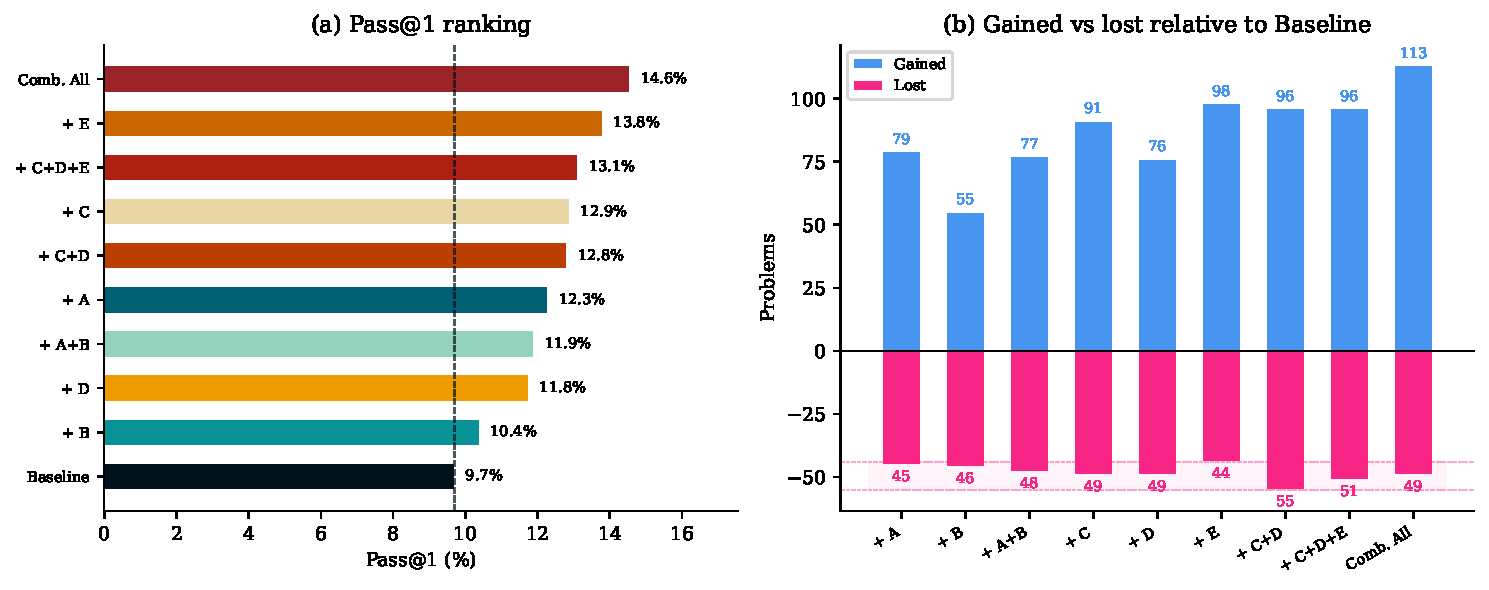
\includegraphics[width=\linewidth]{component/figures/p4/fig2_individual_impact.pdf}
\captionof{figure}{Individual impact of each reward configuration. (a)~Pass@1 ranking; dashed line marks the baseline. (b)~Problems gained (green) and lost (red) vs.\ Baseline; shaded band marks the \pFourLossMin--\pFourLossMax{} loss stability range.}
\label{fig:p4-individual-impact}
\end{minipage}
\vspace{1em}

Number grounding (E) is the strongest individual reward at \pFourSeparateEDeltaPassOne{}pp, followed by non-degeneracy (C, \pFourSeparateCDeltaPassOne{}pp) and format compliance (A, \pFourSeparateADeltaPassOne{}pp); numeric proximity (B) provides only \pFourSeparateBDeltaPassOne{}pp, below our 1\% noise threshold.
E also gains the most problems (\pFourSeparateEGained) with the fewest individual losses (\pFourSeparateELost), yielding the highest individual net (+\pFourSeparateENet).
The full combination achieves the highest Pass@1 (\pFourCombinedAllPassOne\%, \pFourCombinedAllDeltaPassOne{}pp), while C+D+E achieves the highest Pass@8 (\pFourCombinedCdePassEight\%) and lowest extraction failure rate (\pFourCombinedCdeExtrFail\%)---though with the widest Pass@8--Pass@1 gap (\pFourCombinedCdeGap{}pp), indicating breadth without consistency.
Across all ten configurations, the loss count remains remarkably stable at \pFourLossMin--\pFourLossMax{} problems.

\nestunindent
\subsubsection{Interaction Effects}
\nestindent

We compare combined runs against their constituent individual rewards to assess synergy, interference, or additivity.
Figure~\ref{fig:p4-interactions} visualizes the interaction patterns.

\vspace{1em}
\noindent\begin{minipage}{\linewidth}
\centering
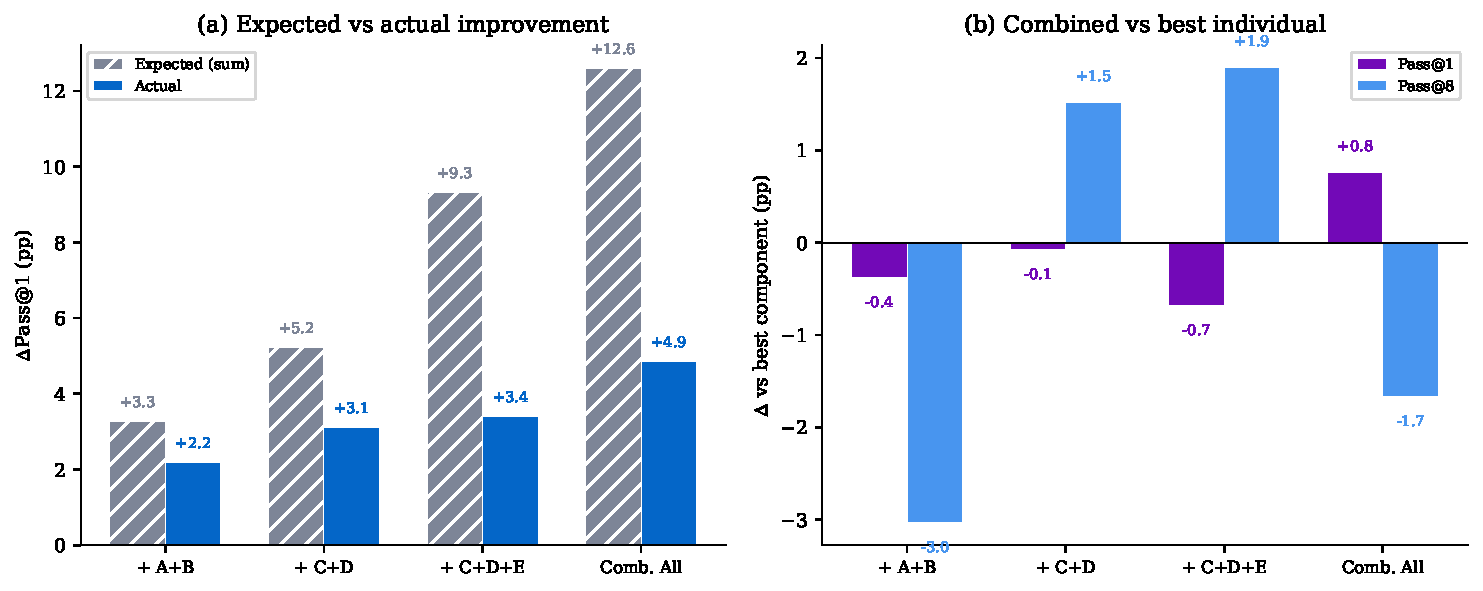
\includegraphics[width=\linewidth]{component/figures/p4/fig3_interactions.pdf}
\captionof{figure}{Reward interaction patterns. (a)~Expected (sum of components) vs.\ actual $\Delta$Pass@1 for each combined run. (b)~$\Delta$ vs.\ best individual component on Pass@1 and Pass@8.}
\label{fig:p4-interactions}
\end{minipage}
\vspace{1em}

A+B (\pFourCombinedAbDeltaPassOne{}pp) underperforms A alone (\pFourSeparateADeltaPassOne{}pp) by 0.4pp, indicating mild interference rather than synergy.
All combined runs are sub-additive: the actual improvement is always less than the sum of individual components.
C+D+E shows the widest gap between expected and actual improvement, yet still achieves the highest Pass@8 of any configuration (\pFourCombinedCdePassEight\%).
The number of gained problems increases with reward count---individual runs gain 55--98 problems, pairs 77--96, and the full combination gains \pFourCombinedAllGained---while losses stay fixed at \pFourLossMin--\pFourLossMax.
Each additional reward unlocks a few extra problems the others miss, so net improvement grows with reward count even though individual contributions overlap.
Despite this sub-additivity, the full combination (\pFourCombinedAllDeltaPassOne{}pp) substantially exceeds any individual reward or pair.

\nestunindent
\subsubsection{Failure Mode Distribution}
\nestindent

We apply the rule-based mistake taxonomy (Table~\ref{tab:taxonomy}) to classify errors across all ten runs.
Table~\ref{tab:p4-errors-full} shows the distribution, and Figure~\ref{fig:p4-error-dist} visualizes the composition shift.

\vspace{1em}
\noindent\begin{minipage}{\linewidth}
\centering
\footnotesize
\captionof{table}{Mistake type distribution across all ten runs. Percentages are within each run's failed set (problems where all 8 samples failed).}
\label{tab:p4-errors-full}
\begin{tabular*}{\linewidth}{@{\extracolsep{\fill}}lrrrrrr}
\toprule
\textbf{Run} & \textbf{No Ans.} & \textbf{Fmt Only} & \textbf{No Reas.} & \textbf{Arith.} & \textbf{Lg.\ Err.} & \textbf{Gibb.} \\
\midrule
Baseline & 273 (27.6\%) & 389 (39.3\%) & 0 & 110 (11.1\%) & 186 (18.8\%) & 32 (3.2\%) \\
\midrule
+ A & 127 (14.4\%) & 153 (17.4\%) & 0 & 173 (19.7\%) & 397 (45.1\%) & 30 (3.4\%) \\
+ B & 244 (25.2\%) & 304 (31.4\%) & 0 & 137 (14.1\%) & 254 (26.2\%) & 30 (3.1\%) \\
+ A+B & 171 (18.6\%) & 190 (20.7\%) & 0 & 177 (19.2\%) & 356 (38.7\%) & 26 (2.8\%) \\
\midrule
+ C & 80 (9.5\%) & 97 (11.5\%) & 0 & 217 (25.8\%) & 438 (52.1\%) & 9 (1.1\%) \\
+ D & 179 (19.5\%) & 240 (26.1\%) & 0 & 161 (17.5\%) & 317 (34.5\%) & 21 (2.3\%) \\
+ E & 53 (6.4\%) & 77 (9.3\%) & 0 & 240 (29.0\%) & 449 (54.2\%) & 9 (1.1\%) \\
+ C+D & 80 (9.7\%) & 73 (8.9\%) & 0 & 205 (25.0\%) & 458 (55.8\%) & 5 (0.6\%) \\
+ C+D+E & 32 (4.0\%) & 51 (6.4\%) & 0 & 220 (27.4\%) & 495 (61.6\%) & 5 (0.6\%) \\
\midrule
Comb.\ All & 76 (8.9\%) & 54 (6.4\%) & 0 & 242 (28.5\%) & 470 (55.3\%) & 8 (0.9\%) \\
\bottomrule
\end{tabular*}
\end{minipage}
\vspace{1em}


\vspace{1em}
\noindent\begin{minipage}{\linewidth}
\centering
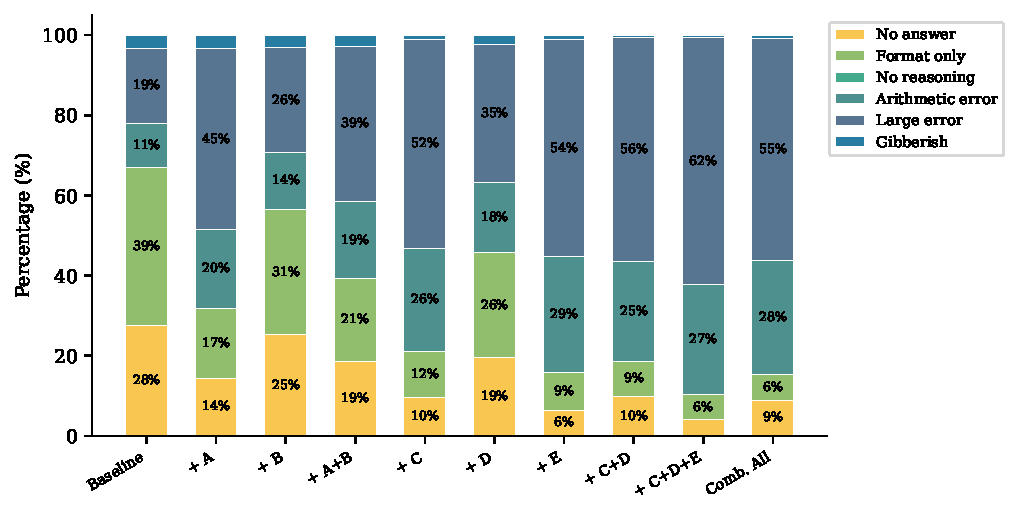
\includegraphics[width=\linewidth]{component/figures/p4/fig4_error_distribution.pdf}
\captionof{figure}{Error category composition (\%) across all runs. The shift from format-related failures (no answer, format only) toward reasoning failures (large error, arithmetic error) is visible across all reward additions.}
\label{fig:p4-error-dist}
\end{minipage}
\vspace{1em}

The baseline's errors are dominated by format failures: ``no answer'' (\pFourBaselineNoAnswer\%) and ``format only'' (\pFourBaselineFormatOnly\%) together account for \pFourBaselineFmtFailPct\%.
Every reward addition shifts this distribution toward reasoning failures (large error, arithmetic error).
Format compliance (A) produces the largest single-reward format reduction (``no answer'' $-$13.1pp, ``format only'' $-$21.9pp), but number grounding (E) achieves comparable or greater reduction---``no answer'' drops to \pFourSeparateENoAnswer\% ($-$21.2pp), ``format only'' to \pFourSeparateEFormatOnly\% ($-$30.0pp)---despite not directly targeting format.
C+D+E nearly eliminates surface-level failures (zero gibberish, lowest format rates at \pFourCombinedCdeNoAnswer\% + \pFourCombinedCdeFormatOnly\%), leaving ``large error'' as the dominant error at \pFourCombinedCdeLargeError\%.
In the full combination, reasoning failures rise to dominate at \pFourCombinedAllReasonPct\%, while format failures shrink to \pFourCombinedAllFmtFailPct\%.

\nestunindent
\subsubsection{Training Dynamics}
\nestindent

We examine per-step training signals logged to W\&B across all 10 runs.
Figure~\ref{fig:p4-training-dynamics} shows mean reward, Pass@1, per-component rewards, and sequence length.

\vspace{1em}
\noindent\begin{minipage}{\linewidth}
\centering
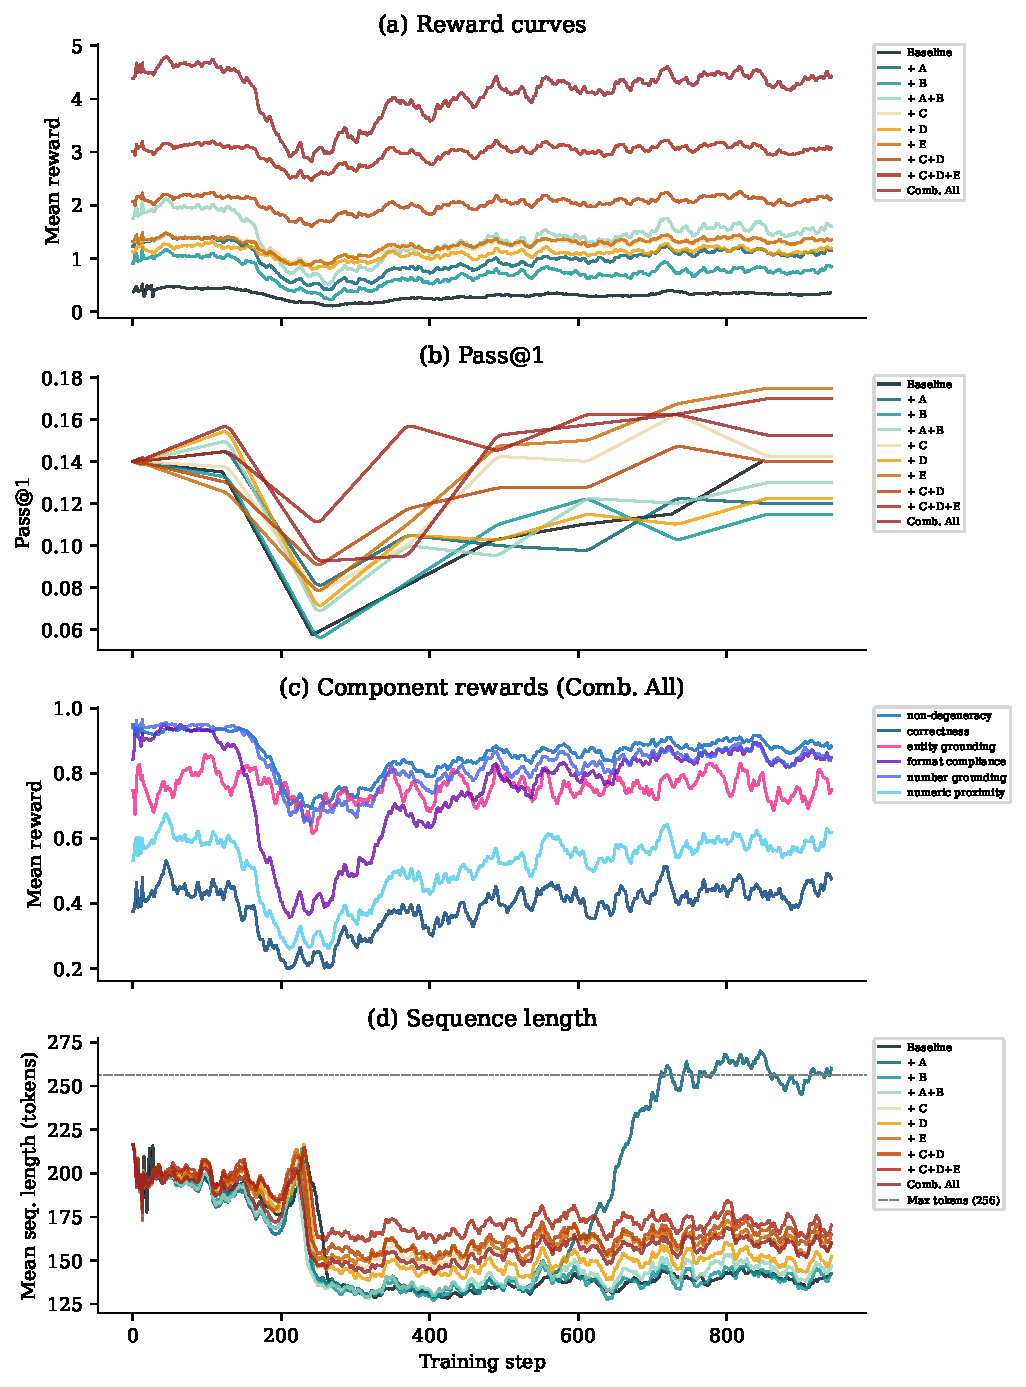
\includegraphics[width=\linewidth]{component/figures/p4/fig5_training_dynamics.pdf}
\captionof{figure}{Training dynamics across all 10 runs. (a)~Mean total reward per step. (b)~Pass@1 over training. (c)~Per-component reward curves for the Comb.\ All run. (d)~Mean sequence length over training.}
\label{fig:p4-training-dynamics}
\end{minipage}
\vspace{1em}

All runs exhibit a sharp initial reward improvement followed by decline, consistent with REINFORCE without KL regularization.
Non-degeneracy (C) is the exception in shape: it peaks late (step 785) with the highest individual correctness at training end (0.473 vs.\ baseline's 0.391), unlike the early-peak-then-decline pattern of format compliance (A) and entity grounding (D).
Proximity (B) is the exception in direction: its correctness component declines below its starting value by training end (0.348).
Format compliance (A) increases sequence length from 216.5 to 276.6 tokens, while all other individual runs decrease; this effect disappears in combinations (A+B: 216.5 $\to$ 154.6).
In the full combination, all five reward components maintain healthy levels at training end (non-degeneracy 0.907, entity grounding 0.830, number grounding 0.874, format 0.867, proximity 0.619) with no single component collapsing, and it ends with the highest correctness (0.461) of any run.

\nestunindent
\nestunindent
